\documentclass[]{article}
\usepackage{amsmath}
\usepackage{graphicx}

\begin{document}

Here, I tried to see the influence of different coding on sub-sampling in logistic regression. 

In the first example, there are 5 continuous variables and 1 categorical variable with 2 levels. 1 dummy variable is used, and it is coded in 2 ways: 1/0 (\textbf{code 1}) and 1/-1 (\textbf{code 2}). Including intercept, there are 7 parameters and the true values are all 0.5 under \textbf{code 1}.

In the second example,  there are 4 continuous variables and 1 categorical variable with 3 levels. 2 dummy variables are used. The three levels are coded in 2 ways: 1)\textbf{code 1}: (1, 0), (0, 1), (0, 0) and 2)\textbf{code 2}: (1, 0), (0, 1), (-1, -1). Again, true values for all 7 parameters are 0.5 under \textbf{code 1}.

The performance of sub-sampling for these 2 cases are summarized in the following 2 plots:

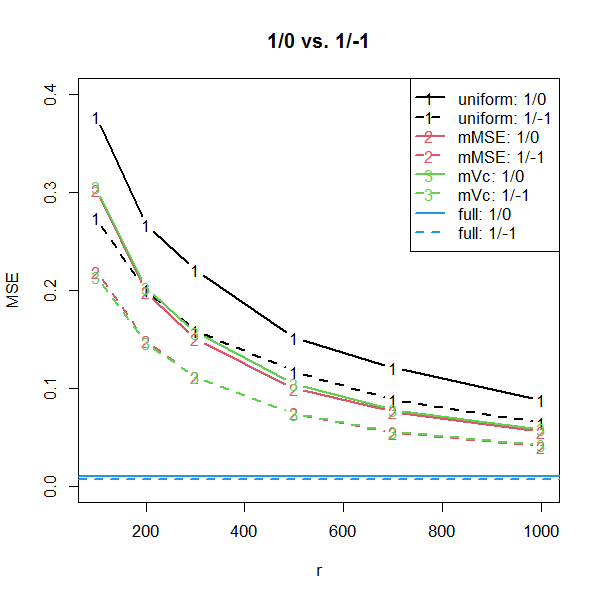
\includegraphics[width = .6\textwidth]{plot_2levels.png}
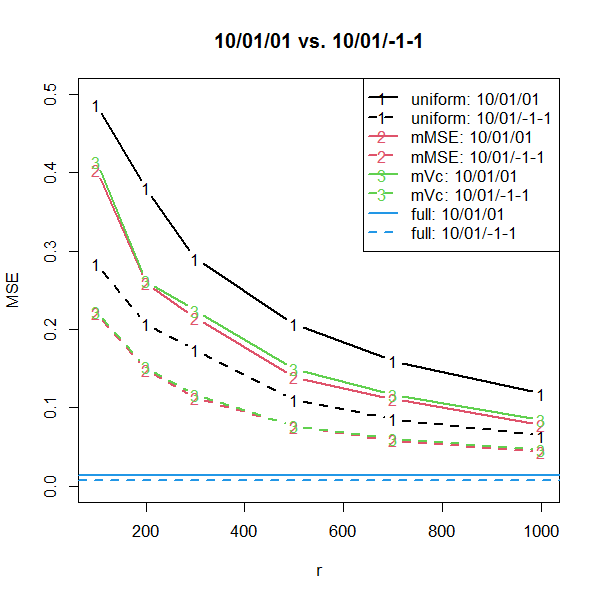
\includegraphics[width = .6\textwidth]{plot_3levels.png}

We can see that including 0 in the coding will reduce the performance of sub-sampling. This is as expected. If we take a look on sub-sampling based on L-optimality criterion:

\begin{equation*}
	\pi_{i}^{mVc} = \frac{|y_i-p_i(\hat{\beta}_MLE)||\boldsymbol{x}_i||}{\sum_{j=1}^{n}|y_i-p_i(\hat{\beta}_MLE)||\boldsymbol{x}_i||}
\end{equation*}

When there exists 0 in $||\boldsymbol{x}_i||$, it will cause problems.




	
	
	
\end{document}


